\documentclass[twoside,twocolumn]{article}

\usepackage{blindtext} % Package to generate dummy text throughout this template 
\usepackage{graphicx}
\usepackage[sc]{mathpazo} % Use the Palatino font
\usepackage[T1]{fontenc} % Use 8-bit encoding that has 256 glyphs
\linespread{1.05} % Line spacing - Palatino needs more space between lines
\usepackage{microtype} % Slightly tweak font spacing for aesthetics

\usepackage[english]{babel} % Language hyphenation and typographical rules

\usepackage[hmarginratio=1:1,top=32mm,columnsep=20pt]{geometry} % Document margins
\usepackage[hang, small,labelfont=bf,up,textfont=it,up]{caption} % Custom captions under/above floats in tables or figures
\usepackage{booktabs} % Horizontal rules in tables

\usepackage{lettrine} % The lettrine is the first enlarged letter at the beginning of the text

\usepackage{enumitem} % Customized lists
\setlist[itemize]{noitemsep} % Make itemize lists more compact

\usepackage{abstract} % Allows abstract customization
\renewcommand{\abstractnamefont}{\normalfont\bfseries} % Set the "Abstract" text to bold
\renewcommand{\abstracttextfont}{\normalfont\small\itshape} % Set the abstract itself to small italic text

\usepackage{titlesec} % Allows customization of titles
\renewcommand\thesection{\Roman{section}} % Roman numerals for the sections
\renewcommand\thesubsection{\roman{subsection}} % roman numerals for subsections
\titleformat{\section}[block]{\large\scshape\centering}{\thesection.}{1em}{} % Change the look of the section titles
\titleformat{\subsection}[block]{\large}{\thesubsection.}{1em}{} % Change the look of the section titles

\usepackage{fancyhdr} % Headers and footers
\pagestyle{fancy} % All pages have headers and footers
\fancyhead{} % Blank out the default header
\fancyfoot{} % Blank out the default footer
\fancyhead[C]{Patrones de Diseño $\bullet$ Octubre 2020 $\bullet$ } % Custom header text
\fancyfoot[RO,LE]{\thepage} % Custom footer text

\usepackage{titling} % Customizing the title section

\usepackage{hyperref} % For hyperlinks in the PDF

%----------------------------------------------------------------------------------------
%	TITLE SECTION
%----------------------------------------------------------------------------------------

\setlength{\droptitle}{-4\baselineskip} % Move the title up

\pretitle{\begin{center}\Huge\bfseries} % Article title formatting
\posttitle{\end{center}} % Article title closing formatting
\title{Patrones de Diseño} % Article title
\author{Arias, Cancino, Crispin, Gutierrez, Zuñiga} 


\date{\today} % Leave empty to omit a date
\renewcommand{\maketitlehookd}{%
\begin{abstract}
	\begin{center}
		\textbf{Resumen}
	\end{center}
	Los patrones de diseño son soluciones a problemas de diseño recurrentes en software científico. Estos patrones se usan para mitigar la ausencia de algunos aspectos de calidad inherentes al software. Los científicos, debido a su formación profesional, abordan diseños poco flexibles y difíciles de mantener en sus aplicaciones. Además, en ausencia de un lenguaje común con ingenieros de software se hace muy compleja la comunicación y validación del dominio de aplicación.  
Normalmente, las representaciones de los patrones de diseño se basan en diagramas de UML u otro tipo de grafos. Estos diagramas son difíciles de entender para los científicos e ingenieros de software inexpertos debido a su nivel de formalismo y, además, porque sólo representan el patrón de diseño aplicado y no el problema genérico que resuelven. Por otro lado, estos diagramas como unidad no poseen los elementos necesarios para representar completamente un dominio de software científico y se deben valer de la combinación de varios de ellos para hacerlo. 
El objetivo de esta investigación es describir lo que es un patrón de diseño, sus objetivos y clasificaciones aportando ejemplos de cada uno de ellos \\
	\begin{center}
		
		\textbf{Abstract}
	\end{center}
	Design patterns are solutions for recurrent design problems in scientific software. These patterns are used to mitigate the lack of several quality aspects inherent in the software. Scientists, due to their professional training, tackle little flexible and maintainable designs for their software applications. In addition, in the absence of a common vocabulary with software engineers, domain communication and validation becomes complex.  
Normally, design patterns representation are based on UML class diagrams or other kind of graphs. These diagrams are difficult to understand for scientist and inexperienced software engineers due to their level of formalism and, also because of this diagrams only represents the implemented design pattern and not the generic problem the design patterns solves. Furthermore, these diagrams as unity do not have the necessary elements to represent scientific software domains completely, so they must combine to do it. 
The objective of this research is to describe what a design pattern is, its objectives and classifications, providing examples of each of them. 
	\\
\end{abstract}
}

%----------------------------------------------------------------------------------------

\begin{document}

% Print the title
\maketitle

%----------------------------------------------------------------------------------------
%	ARTICLE CONTENTS
%----------------------------------------------------------------------------------------

\section{Introduccion}

\lettrine[nindent=0em,lines=3]{U}n patrón de este tipo identifica, abstrae y nombra los aspectos elementales de una estructura de diseño, donde los componentes, son las clases y objetos, y sus mecanismos de interacción son mensajes.  
Cada patrón prescribe una estructura de clases, sus roles y colaboraciones, y una adecuada asignación de métodos para resolver un problema de diseño en una manera flexible y adaptable.  
La aplicación de los patrones en un diseño consiste en identificar el patrón que resuelve el problema de diseño encontrado y aplicar la solución abstracta prescrita por el patrón a dicho problema. 
Uno de los beneficios de utilizar patrones es el entendimiento y documentación de diseños orientados a objetos. Los patrones, también, mejoran el mantenimiento de sistemas ya que proveen una especificación explícita de clases e interacción entre objetos. Además, los patrones proveen un vocabulario para discutir y comunicar decisiones de diseño en término de estructuras de clases en lugar de objetos.  
Los patrones de diseño ayudan a elegir diseños alternativos que hacen un sistema reutilizable y evitan alternativas que comprometan la reutilización  
El libro que ha popularizado los patrones de diseño es el conocido “Design Patterns: Elements of Reusable Object Oriented Software”. En este se recopilan 23 patrones agrupados en tres categorías: de creación, de estructura y de comportamiento.
%------------------------------------------------
%-----------------------------------------------------------------
\section{Desarrollo}
\subsection{ Patrones de Diseño de Software}
La concepción de los patrones de diseño viene de la arquitectura y construcción de edificaciones, donde Alexander et al. (1977) definen que cada patrón describe un problema que ocurre una y otra vez en el tiempo y el elemento principal de una solución que se puede reutilizar sin tener que hacer todo de nuevo.  
En software, los patrones de diseño nacen como una extensión de métodos de análisis y diseño orientados a objetos, para tratar de unificar las soluciones a problemas recurrentes en el desarrollo cotidiano de aplicaciones de software (Gardner, 2004). Estos patrones de diseño conservan la misma esencia que los de Alexander et al. (1977), sólo que, en vez de elementos de arquitectura y construcción de edificaciones, se tienen objetos e interfaces que representan el sistema que se construye (Gamma et al., 1994).  
Gamme et al. (1994) introducen la primera formalización de los patrones de diseño, al definir los elementos principales de un patrón de diseño genérico: 

\begin{itemize}
	\item \textbf{El nombre del patrón:} define en una palabra o dos el problema de diseño, la intención de la solución y las consecuencias de su uso.  
	\item \textbf{El problema:} define las condiciones del problema que soluciona, en algunos casos mediante listas de chequeo o la definición de un contexto.  
	\item \textbf{La solución:} describe las entidades, relaciones y responsabilidades que componen la solución. Usualmente, se representa a partir de diagramas de UML e incluye una plantilla que se puede aplicar a varios contextos o dominios de aplicación.  
	\item \textbf{Las consecuencias:} describen el resultado de un diseño basado en el patrón de diseño y cómo afecta al resto del diseño del sistema. 
\end{itemize}
Los patrones de diseño se definieron y crearon especialmente para paradigmas orientados a objetos. El desempeño e implementación dependen directamente del lenguaje de programación y, en algunos casos, del contexto donde se usen (Shalloway y Trott, 2004).  
La representación de estos patrones se basa, en la mayoría de los casos, en notaciones gráficas usando diagramas de UML y, en algunas ocasiones, en otro tipo de grafos. Además, la definición de cada patrón de diseño debe contener unas secciones de soporte para facilitar el entendimiento de dicho patrón: el nombre del patrón de diseño y su clasificación, motivación, aplicabilidad, estructura, participantes, colaboraciones y consecuencias. Finalmente, esta representación sólo expresa el estado final del patrón de diseño aplicado y sólo se enfoca en la estructura resultante de la implementación (Gamma et al., 1994).  
Gamma et al.(1994) definen, en total, 23 patrones de diseño donde se resaltan las mayores premisas del diseño de software: composición sobre herencia, bajo acoplamiento, alta cohesión y correcta asignación de responsabilidades. Estos patrones de diseño se distribuyen en tres categorías: patrones de diseño estructurales, de comportamiento y de creación. 

\subsection{Patrones de diseño de creación}
Los Patrones de Diseño de Creación se enfocan en hacer un sistema independiente de la manera en que sus objetos y clases se crean, componen y representan. Estos patrones resumen el proceso de creación o instanciación de estos elementos (Gamma et al., 1994). Existen dos aproximaciones: a nivel de clases y a nivel objetual. Los patrones de diseño de creación a nivel de clases usan la generalización para variar la clase que se está instanciando. Por otro lado, a nivel objetual, se delega el proceso de instanciación de un objeto a otro (Shalloway y Trott, 2004) 
Los patrones de diseño de creación se enfocan principalmente en el principio de diseño de composición sobre herencia, el cual toma relevancia a medida que el sistema evoluciona y crece (Gamma et al., 1994). Los patrones de diseño de creación se listan y definen (Pree y Sikora, 1995; Stelting y Maassen, 2002) a continuación: 	

\begin{itemize}

    \item \textbf{Patrones de diseño creacionales} 
    Son patrones de diseño que se ocupan de los mecanismos de creación de objetos, tratando de crear objetos de manera adecuada a la situación. La forma básica de creación de objetos podría ocasionar problemas de diseño o agregar complejidad al diseño. Los patrones de diseño creacionales resuelven este problema controlando de alguna manera la creación de este objeto.
    \begin{itemize}
		\item \textbf{Abstract Factory:}	este patrón de diseño provee una interfaz o una clase abstracta, la cual define la creación de una familia de objetos relacionados o dependientes sin especificar su clase de origen. 
		\item \textbf{Builder:} el Builder se enfoca en la creación de objetos complejos. Este patrón separa el proceso de construcción del objeto de su implementación, logrando así usar el mismo proceso de creación para otras representaciones del mismo objeto.  
		\item \textbf{Factory Method:} el patrón Factory Method define una interfaz genérica para la creación de un objeto. Este patrón de diseño trabaja a nivel de clases y le permite a una subclase instanciar la clase adecuada para el contexto definido.  
		\item \textbf{Prototype:}	este patrón define una estructura deseada para el objeto y permite instanciar objetos haciendo una copia de éste.  
		\item \textbf{Singleton:} el patrón Singleton restringe el número de instancias de una clase a sólo una en todo el sistema. 
    \end{itemize}

    %%-------------------------------
	\item \textbf{PATRON SINGLETON}
	\begin{itemize}
		\item \textbf{Intención:}	Garantiza que una clase sólo tenga una instancia y proporciona un punto de acceso global a ella. 

		\item \textbf{Problema:} Varios clientes distintos precisan referenciar a un mismo elemento y queremos asegurarnos de que no hay más de una instancia de ese elemento. 

		\item \textbf{Solución :} Garantizar una única instancia. 
			\begin{center}
			    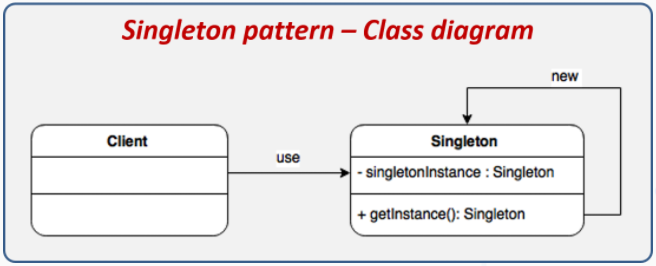
\includegraphics[width=5cm]{./img/imagen1.png} 
            \end{center}
		\item \textbf{Participantes :}	
        \begin{itemize}
        \item \textbf{Singleton:}	
            \begin{itemize}
                \item Define una operación Instancia que permite que los clientes accedan a su única instancia. Instancia es una operación de clase (static en C# y shared en VB .NET). 	
                \item Puede ser responsable de crear su única instancia.  	
            \end{itemize}
        \end{itemize}    

		\item \textbf{Aplicabilidad :} Usar cuando: 
        \begin{itemize}
            \item Deba haber exactamente una instancia de una clase y ésta deba ser accesible a los clientes desde un punto de acceso conocido.  	
            \item La única instancia debería ser extensible mediante herencia y los clientes deberían ser capaces de utilizar una instancia extendida sin modificar su código. 	
        \end{itemize}

		\item \textbf{Consecuencias:} 
        \begin{itemize}
            \item Acceso controlado a la única instancia. Puede tener un control estricto sobre cómo y cuando acceden los clientes a la instancia.   	
            \item Espacio de nombres reducido. El patrón Singleton es una mejora sobre las variables globales. 	   
            \item Permite el refinamiento de operaciones y la representación. Se puede crear una subclase de Singleton.   
            \item Permite un número variable de instancias. El patrón hace que sea fácil cambiar de opinión y permitir más de una instancia de la clase Singleton.  	
        \end{itemize}
	\end{itemize}
	
	\item \textbf{DIAGRAMA DE CLASES}
    \begin{center}
        \includegraphics[width=5cm]{./img/imagen2.png} 
    \end{center}
    \\
    Los componentes que conforman el patrón son los siguientes: 
	\begin{itemize}
		\item \textbf{Client:} Componente que desea obtener una instancia de la clase Singleton. 
		\item \textbf{Singleton:} Clase que implementa el patrón Singleton, de la cual únicamente se podrá tener una instancia durante toda la vida de la aplicación. 
    \end{itemize}
    \item \textbf{DIAGRAMA DE ARQUITECTURA}
    \begin{center}
        \includegraphics[width=5cm]{./img/imagen3.png} 
    \end{center}
    \\
    \item \textbf{EJEMPLO DE IMPLEMENTACIÓN}
    \begin{center}
        \includegraphics[width=5cm]{./img/imagen4.png} 
    \end{center}
	
    \item \textbf{Patrones de diseño estructurales  }
	\\
	\\Son patrones de diseño que se ocupan de los mecanismos de creación de objetos, tratando de crear objetos de manera adecuada a la situación. La forma básica de creación de objetos podría ocasionar problemas de diseño o agregar complejidad al diseño. Los patrones de diseño creacionales resuelven este problema controlando de alguna manera la creación de este objeto.\cite{Tanembaum2}
	\begin{itemize}
		\item \textbf{Adapter:}	el patrón Adapter le permite a un cliente trabajar con clases cuya interfaz no posee una interfaz permitida en un sistema específico. Este patrón adapta la interfaz del objeto externo al de las clases del sistema al que se integra.  
		\item \textbf{Bridge:} este patrón desacopla la abstracción de una clase de su implementación, permitiendo así, que varíen independientemente y se entregue flexibilidad y facilidad de mantenimiento al software.  
		\item \textbf{Composite:} el patrón Composite compone objetos relacionados en una jerarquía de tipo árbol. Este patrón de diseño le permite al cliente tratar de la misma manera un objeto y un grupo de objetos. 
		\item \textbf{Decorator:}	el patrón de diseño Decorator le añade responsabilidades adicionales a un objeto en tiempo de ejecución.  
		\item \textbf{Flyweight:}  este patrón de diseño permite apoyarse en la copia de objetos complejos en un sistema que requiere la instanciación de un gran número de objetos con una estructura similar.  
		\item \textbf{Facade:} este patrón provee una interfaz que representa las interfaces de los subsistemas del software. Además, facilita el uso de un sistema complejo con muchas relaciones directas al cliente.  
		\item \textbf{Proxy:} el patrón Proxy restringe el acceso a un objeto para evitar su creación o participación precoz en el sistema. Usualmente, trata a objetos complejos o de gran tamaño. 
        \\
        \\
    \end{itemize}

    %%-------------------------------
    \item \textbf{PATRON DECORATOR} \\
    El patrón decorator está diseñado para solucionar problemas donde la jerarquía con subclasificación no puede ser aplicada, o se requiere de un gran impacto en todas las clases de la jerarquía con el fin de poder lograr el comportamiento esperado. Decorator permite al usuario añadir nuevas funcionalidades a un objeto existente sin alterar su estructura, mediante la adición de nuevas clases que envuelven a la anterior dándole funcionamiento extra. 
	\begin{itemize}
		\item \textbf{OBJETIVO :}	Su función es determinar como las clases y objetos se combinan para formar estructuras.
        Estas estructuras permitirán que se agreguen nuevas funcionalidades.
        
        \begin{center}
            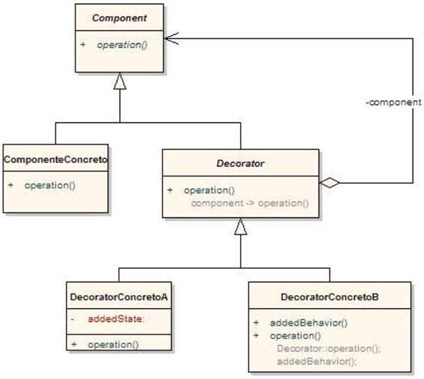
\includegraphics[width=5cm]{./img/Imagen5.png} 
        \end{center}
        \\

		\item \textbf{MOTIVACIÓN  :} Dotar de funcionalidades dinámicamente a objetos mediante composición. Es decir, vamos a decorar los objetos para darles más funcionalidad de la que tienen en un principio.
        Esto es algo verdaderamente útil cuándo queremos evitar jerarquías de clases complejas. La herencia es una herramienta poderosa, pero puede hacer que nuestro diseño sea mucho menos extensible.
        

		\item \textbf{APLICACIONES  :} \\
        El patrón se utiliza en los casos siguientes: 
            \begin{itemize}
                \item Añadir responsabilidades a objetos individuales de forma dinámica y transparente   	
                \item Responsabilidades de un objeto pueden ser retiradas	   
                \item Cuando la extensión mediante la herencia no es viable   
                \item Hay una necesidad de extender la funcionalidad de una clase, pero no hay razones para extenderlo a través de la herencia.  	
                \item Existe la necesidad de extender dinámicamente la funcionalidad de un objeto y quizás quitar la funcionalidad extendida.
            \end{itemize}
            \begin{center}
			    \includegraphics[width=5cm]{./img/imagen6.png} 
            \end{center}
            \begin{itemize}
                \item El Cliente realiza una operación sobre el DecoratorA.   	
                \item El DecoratorA realiza la misma operación sobre DecoradorB.   
                \item El decoradorB realiza una acción sobre ConcreteComponente. 
                \item El DecoradorB ejecuta una operación de decoración.  	
                \item El DecoradorA ejecuta una operación de decoración.	
                \item El Cliente recibe como resultado un objeto decorado por todos los Decoradores, los cuales encapsularon el Component en varias capas.
            \end{itemize}
		   
	\end{itemize}
	
	\item \textbf{DIAGRAMA DE ARQUITECTURA :}	\\
        Mediante la implementación del patrón de diseño Decorator crearemos una aplicación que nos permite procesar un mensaje en capas, donde cada capa se encargará de procesar un mensaje a diferente nivel.
        
        \begin{center}
            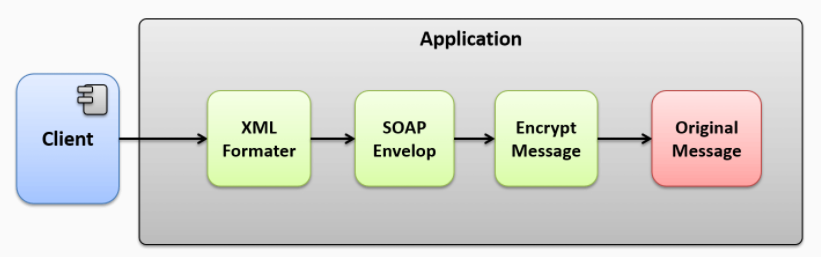
\includegraphics[width=5cm]{./img/Imagen7.png} 
        \end{center}
        \\

        \begin{itemize}
        \item \textbf{EJEMPLO DE IMPLEMENTACION:}	
        
        \begin{center}
            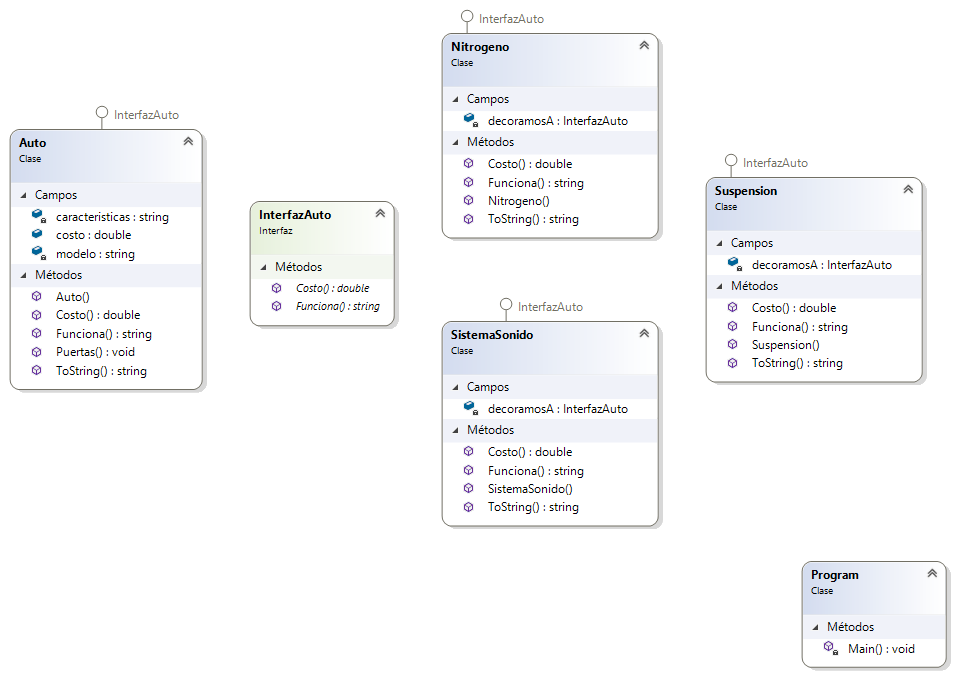
\includegraphics[width=5cm]{./img/Imagen8.png} 
        \end{center}
        \\

        \end{itemize} 

	
    \item \textbf{Patrones de Diseño de Comportamiento }
	\\
	\\Los patrones de Diseño de Comportamiento se enfocan en la asignación de responsabilidades entre clases y objetos (Shalloway y Trott, 2004). 
    Estos patrones determinan flujos de control y comunicación complejos entre objetos que de otra forma, sería complejo seguir en tiempo de ejecución (Stelting y Maassen, 2002). Estos patrones de diseño distribuyen, a nivel de clase, el comportamiento y las responsabilidades. Por otro lado, a nivel objetual, se describe la colaboración entre objetos para cumplir con una tarea común (Gamma et al., 1994). La descripción de estos patrones (Gamma et al., 1994; Stelting y Maassen, 2002) se lista a continuación:
    
	\begin{itemize}
		\item \textbf{Chain of responsibility:}	el propósito de este patrón de diseño es evitar el acoplamiento entre el objeto receptor y emisor de un mensaje específico. El patrón transfiere la responsabilidad a un objeto disponible.  
		\item \textbf{Command:} este patrón encapsula una petición como un objeto para permitir su parametrización.   
		\item \textbf{Interpreter:} el patrón Interpreter, dado un lenguaje, permite definir una representación para su gramática y solucionar el mismo problema recurrente desde el contexto al que pertenece.  
		\item \textbf{Iterator:}	este patrón de diseño proporciona una manera de acceder a un objeto agregado sin exponer su estructura interna.  
		\item \textbf{Mediator:}  el patrón de diseño Mediator permite el bajo acople entre un conjunto de clases asignándole la implementación de los métodos a una sola clase.   
		\item \textbf{Memento:} este patrón de diseño captura y externaliza el estado interno de un objeto para que éste pueda variar y volver al estado inicial en cualquier tiempo.   
		\item \textbf{State:} el patrón de diseño State permite a un objeto cambiar su comportamiento con base en los cambios de su estado interno.  
        \item \textbf{Strategy:} este patrón de diseño permite encapsular algoritmos o funcionalidades específicas y hacerlas intercambiables. Este patrón de diseño le permite al algoritmo variar sin depender del cliente.  
        \item \textbf{Template Method:} el patrón de diseño Template Method define el esqueleto de un algoritmo y permite cambiar ciertos pasos del mismo en las subclases. Estos cambios no afectan al algoritmo original.  
        \item \textbf{Visitor:} este patrón de diseño permite adicionar funcionalidades a una clase existente sin afectar su estructura. 
        \item \textbf{Observer:} el patrón de diseño Observer define una dependencia de uno a muchos entre un conjunto de objetos para actualizarlos automáticamente una vez el objeto principal cambie su estado interno. 
        \\
        \\
    \end{itemize}


    %%-------------------------------
    \item \textbf{PATRON ITERATOR} \\
    Es un mecanismo de acceso a los elementos que constituyen una estructura de datos para la utilización de estos sin exponer su estructura interna. 
    El patrón Iterator proporciona un acceso secuencial a una colección de objetos a los clientes sin que éstos tengan que preocuparse de la implementación de esta colección. 
    
	\begin{itemize}
		\item \textbf{OBJETIVO :}	Proporcionar una forma de acceder a los elementos de una colección de objetos de manera secuencial sin revelar su representación interna. 
        Define una interfaz que declara métodos que permitan acceder secuencialmente a la colección. 
         
        \begin{center}
            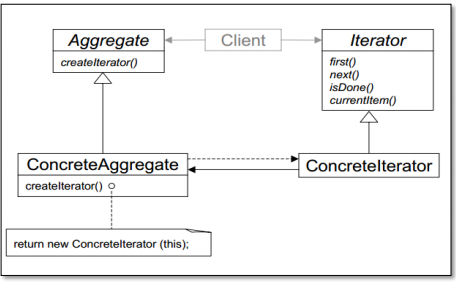
\includegraphics[width=5cm]{./img/Imagen9.png} 
        \end{center}
        \\
		\item \textbf{MOTIVACIÓN  :} El patrón surge del deseo de acceder a los elementos de un contenedor de objetos (por ejemplo, una lista) sin exponer su representación interna. Además, es posible que se necesite más de una forma de recorrer la estructura siendo para ello necesario crear modificaciones en la clase. 
        La solución que propone el patrón es añadir métodos que permitan recorrer la estructura sin referenciar explícitamente su representación. La responsabilidad del recorrido se traslada a un objeto iterador.  
        El problema de introducir este objeto iterador reside en que los clientes necesitan conocer la estructura para crear el iterador apropiado
         

		\item \textbf{APLICACIONES  :} El patrón se utiliza en los casos siguientes:  
            \begin{itemize}
            \item Es necesario realizar un recorrido de acceso al contenido de una colección sin acceder a la representación interna de esta colección. 
            \item Debe ser posible gestionar varios recorridos de forma simultánea.
            \end{itemize}   
        
            
		\item \textbf{CONSECUENCIAS  :}	Los iteradores simplifican la interfaz de las colecciones, ya que la interfaz de los recorridos se encuentra en los iteradores y no en la clase que corresponde a la estructura en cuestión. 
        Permite variaciones en el recorrido de una colección. 
        Para cambiar el algoritmo de recorrido basta cambiar la instancia de Iterator concreta  Nuevos recorridos mediante nuevas subclases de Iterator  
        Se puede tener más de un recorrido en progreso al mismo tiempo por cada colección
        
        
	\end{itemize}
	
	\item \textbf{DIAGRAMA DE CLASES :}	\\
    Los métodos más comunes son:

    \begin{itemize}
        \item \textbf{hasNext  :} Método que regresa un booleano para indicar si existen más elementos en la estructura por recorrer. True si existen más y false si hemos llegado al final y no hay más elementos por recorrer.
        \item \textbf{next  :} Regresa el siguiente elemento de la estructura de datos.
        \end{itemize} 

        \begin{center}
            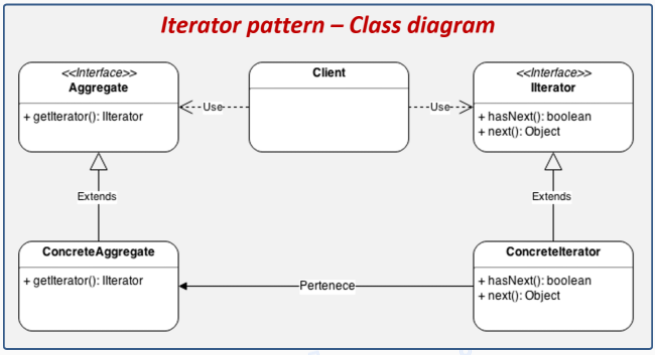
\includegraphics[width=5cm]{./img/Imagen10.png} 
        \end{center}
        \\
        Los elementos del patrón Iterator se describen a continuación:

        \begin{itemize}
            \item \textbf{Client  :} Actor que utiliza al Iterator.
            \item \textbf{Aggregate  :} Interface que define la estructura de las clases que pueden ser iteradas.
            \item \textbf{ConcreteAggregate  :} Clase que contiene la estructura de datos que deseamos iterar.
            \item \textbf{IIterator  :} Interface que define la estructura de los iteradores, la cual define los métodos necesarios para poder realizar la iteración sobre el ConcreteAggregator.
            \item \textbf{ConcreteIterator  :} Implementación de un iterador concreto, el cual hereda de IIterator para implementar de forma concreta cómo iterar un ConcreteAggregate.
            \end{itemize} 


        \begin{itemize}
        \item \textbf{DIAGRAMA DE ARQUITECTURA:}	\\
        Patrón de diseño Iterator crearemos una aplicación que nos permita recorrer una estructura organizacional jerárquica, mediante la implementación de un iterador, el cual nos permitirá recorrer todo el árbol de la estructura de forma secuencial.
        \begin{center}
            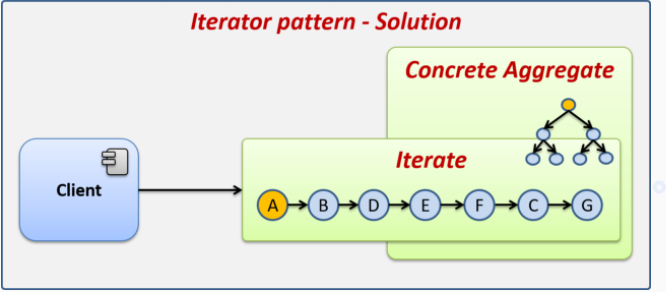
\includegraphics[width=5cm]{./img/Imagen11.png} 
        \end{center}
        \\

        \end{itemize} 

    \item \textbf{EJEMPLO DE IMPLEMENTACIÓN}
    \begin{center}
        \includegraphics[width=5cm]{./img/imagen12.png} 
    \end{center}
	

    %%-------------------------------
\section{Conclusiones}
\begin{itemize}
    En este artículo se ha pretendido introducir al lector en el mundo de los patrones software, pero partiendo desde la perspectiva inicial de este concepto.
    Se ha buscado familiarizar al lector con el concepto de patrón, con sus características y sus peculiaridades, más que con su utilización en el ámbito del Diseño Orientado a Objeto para construir aplicaciones software, con el fin de evitar caer en los falsos mitos y errores, causados por el desconocimiento y la falta de comprensión, propios de un acercamiento poco exhaustivo a una nueva área de conocimiento. 
    Se ha querido recoger en este artículo una amplia lista de referencias, a las que cualquier lector interesado pueda acceder para profundizar más en este interesante campo.
\end{itemize}


\section{Recomendaciones}
\begin{itemize}
	Al desarrollar aplicaciones robustas y fáciles de mantener, debemos cumplir ciertas “reglas”. Lo pongo entre comillas porque aunque estas reglas de diseño son recomendables (muy recomendables), no son obligatorias. Siempre podemos decidir no aplicarlas. Aunque si no lo hacemos, hay que ser conscientes de la razón de no aplicarlas y de sus consecuencias.
Los patrones de diseño nos ayudan a cumplir muchos de estos principios o reglas de diseño. Programación SOLID, control de cohesión y acoplamiento o reutilización de código son algunos de los beneficios que podemos conseguir al utilizar patrones.

\end{itemize}



%------------------------------------------------
%-----------------------------------------------------------------
\section{Bibliografía}\label{sec:6}
\begin{itemize}
\item Coplien, James O. and Schmidt, Douglas (editors). “Pattern Languages of Program Design”. Addison-Wesley. 1995.(2015)
\item Appleton, Brad. “Patterns and Software: Essential Concepts and Terminology”. http://www.enteract.com/~bradapp \\ /docs/patterns-intro.html. November 1997.(2016)
\item López Tallón, Alberto. “Patrones de Diseño. Reutilización de Ideas”. Revista Profesional para Programadores (RPP). Nº43: 54-58. Septiembre, 1998.
\item Gamma, Erich, Helm, Richard, Johnson, Ralph and Vlissides, John. “Design Patterns. Elements of Reusable Object-Oriented Software”. Addison-Wesley, 1995.
\item Source Making. (2015). Singleton Design Pattern. Recuperado de https://sourcemaking.com/design\_ \\ patterns/singleton
\item Tutorials Point. (2016). Design Pattern - Singleton Pattern. Recuperado de https://www.tutorialspoint.com/ \\ design\_pattern/singleton\_pattern.htm
\item Ortega Mateo, Ezequiel. (2020). Patrón estructural - DECORATOR. Viernes, 24 Abril, de SOMOSPNT Sitio web: https://somospnt.com/blog/160-patron-estructural-decorator
\item Gustavo. (2019). Patrón de Diseño Decorator en Java. Mayo 10 , de Experto.dev Sitio web: https://experto.dev/patron-de-diseno-decorator-en-java/
\item RUBENFA. (2014). Patrones de diseño: Decorator. 30 Octubre, de GENBETA:dev Sitio web: https://www.genbeta.com/desarrollo \\ /patrones-de-diseno-decorator
\end{itemize}
% Bibliografia.
%-----------------------------------------------------------------

\bibliographystyle{plain}
\bibliography{bibliografia}
\end{document}
